\documentclass[aspectratio=169]{beamer}
\usepackage[utf8]{inputenc}

% design
\usetheme{CambridgeUS}
\usecolortheme{beaver}
\setbeamertemplate{itemize items}[square]
\usenavigationsymbolstemplate{\beamertemplatenavigationsymbolsempty}
\definecolor{darkred}{rgb}{0.8,0,0}
\colorlet{grey1}{gray!10!white} % I think = RGB 0.95 0.95 0.95
\colorlet{grey2}{gray!60!white} % I think = RGB 0.7 0.7 0.7
\setbeamertemplate{enumerate item}{\color{darkred}\insertenumlabel.}
\setbeamertemplate{itemize item}{\color{darkred}$\blacktriangleright$}
\setlength{\tabcolsep}{12pt}
\setbeamercolor{block title}{fg=darkred}

% bibliography
%\usepackage[backend=biber, style=authortitle]{biblatex}
\usepackage{natbib}
\usepackage{har2nat}
\bibliographystyle{unsrt}
%\addbibresource{../../smc.bib}
\usepackage{bibentry}
\nobibliography*

% tikz
\usepackage{tikz}
\usetikzlibrary{positioning}

% maths
\usepackage{amsmath}
\usepackage{amssymb}
\usepackage{amsfonts}
\usepackage{amsthm}
\theoremstyle{definition}
\newtheorem{defn}{Definition}

% useful math symbols
\newcommand{\PR}{\mathbb{P}}
\newcommand{\E}{\mathbb{E}}
\newcommand{\V}{\operatorname{Var}}
\newcommand{\eqdist}{\overset{d}{=}}
\newcommand{\I}[1]{\mathbb{I}\{#1\}}
\newcommand{\Ntoinfty}{\overset{N\to\infty}{\longrightarrow}}
\newcommand{\limNtoinfty}{\underset{N\to\infty}{\lim}}
\newcommand\indep{\protect\mathpalette{\protect\independenT}{\perp}}
\def\independenT#1#2{\mathrel{\rlap{$#1#2$}\mkern2mu{#1#2}}}

% distributions
\newcommand{\N}{\mathcal{N}}
\newcommand{\Cat}{\operatorname{Categorical}}
\newcommand{\Unif}{\operatorname{Uniform}}
\newcommand{\Mn}{\operatorname{Multinomial}}
\newcommand{\Bin}{\operatorname{Binomial}}

% project-specific commands
\newcommand{\F}{\mathcal{F}_{t-1}}
%\newcommand{\vt}[2][t]{v_{#1}^{(#2)}}
\newcommand{\vt}[1]{v_{#1}}
%\newcommand{\wt}[2][t]{w_{#1}^{(#2)}}
\newcommand{\wt}[1]{w_{#1}}
%\newcommand{\wbar}[2][t]{\bar{w}_{#1}^{(#2)}}
%\newcommand{\vttilde}[2][t]{\tilde{v}_{#1}^{(#2)}}

\title[SMC genealogies]{Genealogies of sequential Monte Carlo algorithms}
\author{Suzie Brown}
\date{27 October 2020}

\begin{document}
\begin{frame}
\maketitle
\end{frame}


\begin{frame}{Outline}
\begin{enumerate}
\item Sequential Monte Carlo
\item Resampling and degeneracy
\item Genealogies
\end{enumerate}
\end{frame}


\begin{frame}{Sequential Monte Carlo}
\begin{itemize}
\item Want to sample from a sequence of intractable target distributions
\item Typical settings: dimension of target increases in time, strong dependence between consecutive targets (so MCMC is impractical)
\item SMC can obtain exact draws, and thus approximate expectations
\end{itemize}

%%% NOTES
% Typically the sequence is indexed by time
% Run-time is linear in number of dimensions, cf MCMC
% Dependence between consecutive targets is a help rather than a hindrance, cf MCMC
% Inference can be done on-line
% Most stuff you might want to know about Bayes posterior can be written as an expectation
\end{frame}


\begin{frame}{State space models}
\begin{columns}
\begin{column}{0.45\textwidth}
\begin{center}
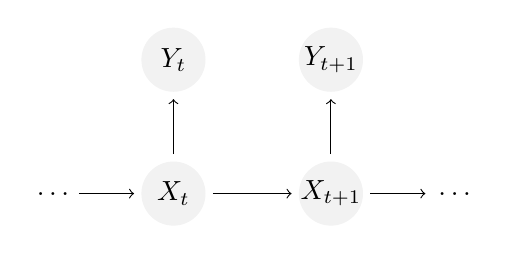
\begin{tikzpicture}
\filldraw[grey1] (0,0) circle (0.4);
\filldraw[grey1] (0,1.7) circle (0.4);
\filldraw[grey1] (2,0) circle (0.4);
\filldraw[grey1] (2,1.7) circle (0.4);
\node at (2,1.7) {$Y_{t+1}$};
\node at (2,0) {$X_{t+1}$};
\node at (0,1.7) {$Y_{t}$};
\node at (0,0) {$X_{t}$};
\node at (-1.5,0) {$\dots$};
\node at (3.6,0) {$\dots$};
\draw[->] (-1.2,0)--(-0.5,0);
\draw[->] (0.5,0)--(1.5,0);
\draw[->] (2.5,0)--(3.2,0); 
\draw[->] (0,0.5)--(0,1.2);
\draw[->] (2,0.5)--(2,1.2);
\end{tikzpicture}
\end{center}
\begin{align*}
& X_0 \sim \mu(\cdot) \\
& X_{t+1} \mid (X_t = x_t) \sim f_t(\cdot | x_t)\\
& Y_t \mid (X_t = x_t) \sim g_t(\cdot | x_t)
\end{align*}
\end{column}
\begin{column}{0.45\textwidth}
May want to infer ($t<T$):

\renewcommand{\arraystretch}{1.5}
\begin{tabular}{l l}
$p(x_{1:T} \mid y_{1:t})$ & ``prediction'' \\
$p(x_{1:t} \mid y_{1:t})$ & ``filtering'' \\
$p(x_{1:t} \mid y_{1:T})$ & ``smoothing''
\end{tabular}
\end{column}
\end{columns}

%%% NOTES
% Flexible class of models much used in applications
% Helpful for illustrating SMC
%-
% X = hidden states we want to infer
% Y = (noisy) observations
%-
% Intractable except in a few special cases
% Examples: stochastic volatility, target tracking
\end{frame}

%\begin{frame}{Example: sleep monitoring}
%\begin{itemize}
%\item $X_t$ encodes the patient's state awake/asleep
%\item $Y_t$ is a vector of observations, say heart rate and body temperature
%\item Want to infer how well the patient slept over the whole night $\rightarrow$ smoothing
%\end{itemize}
%\centering
%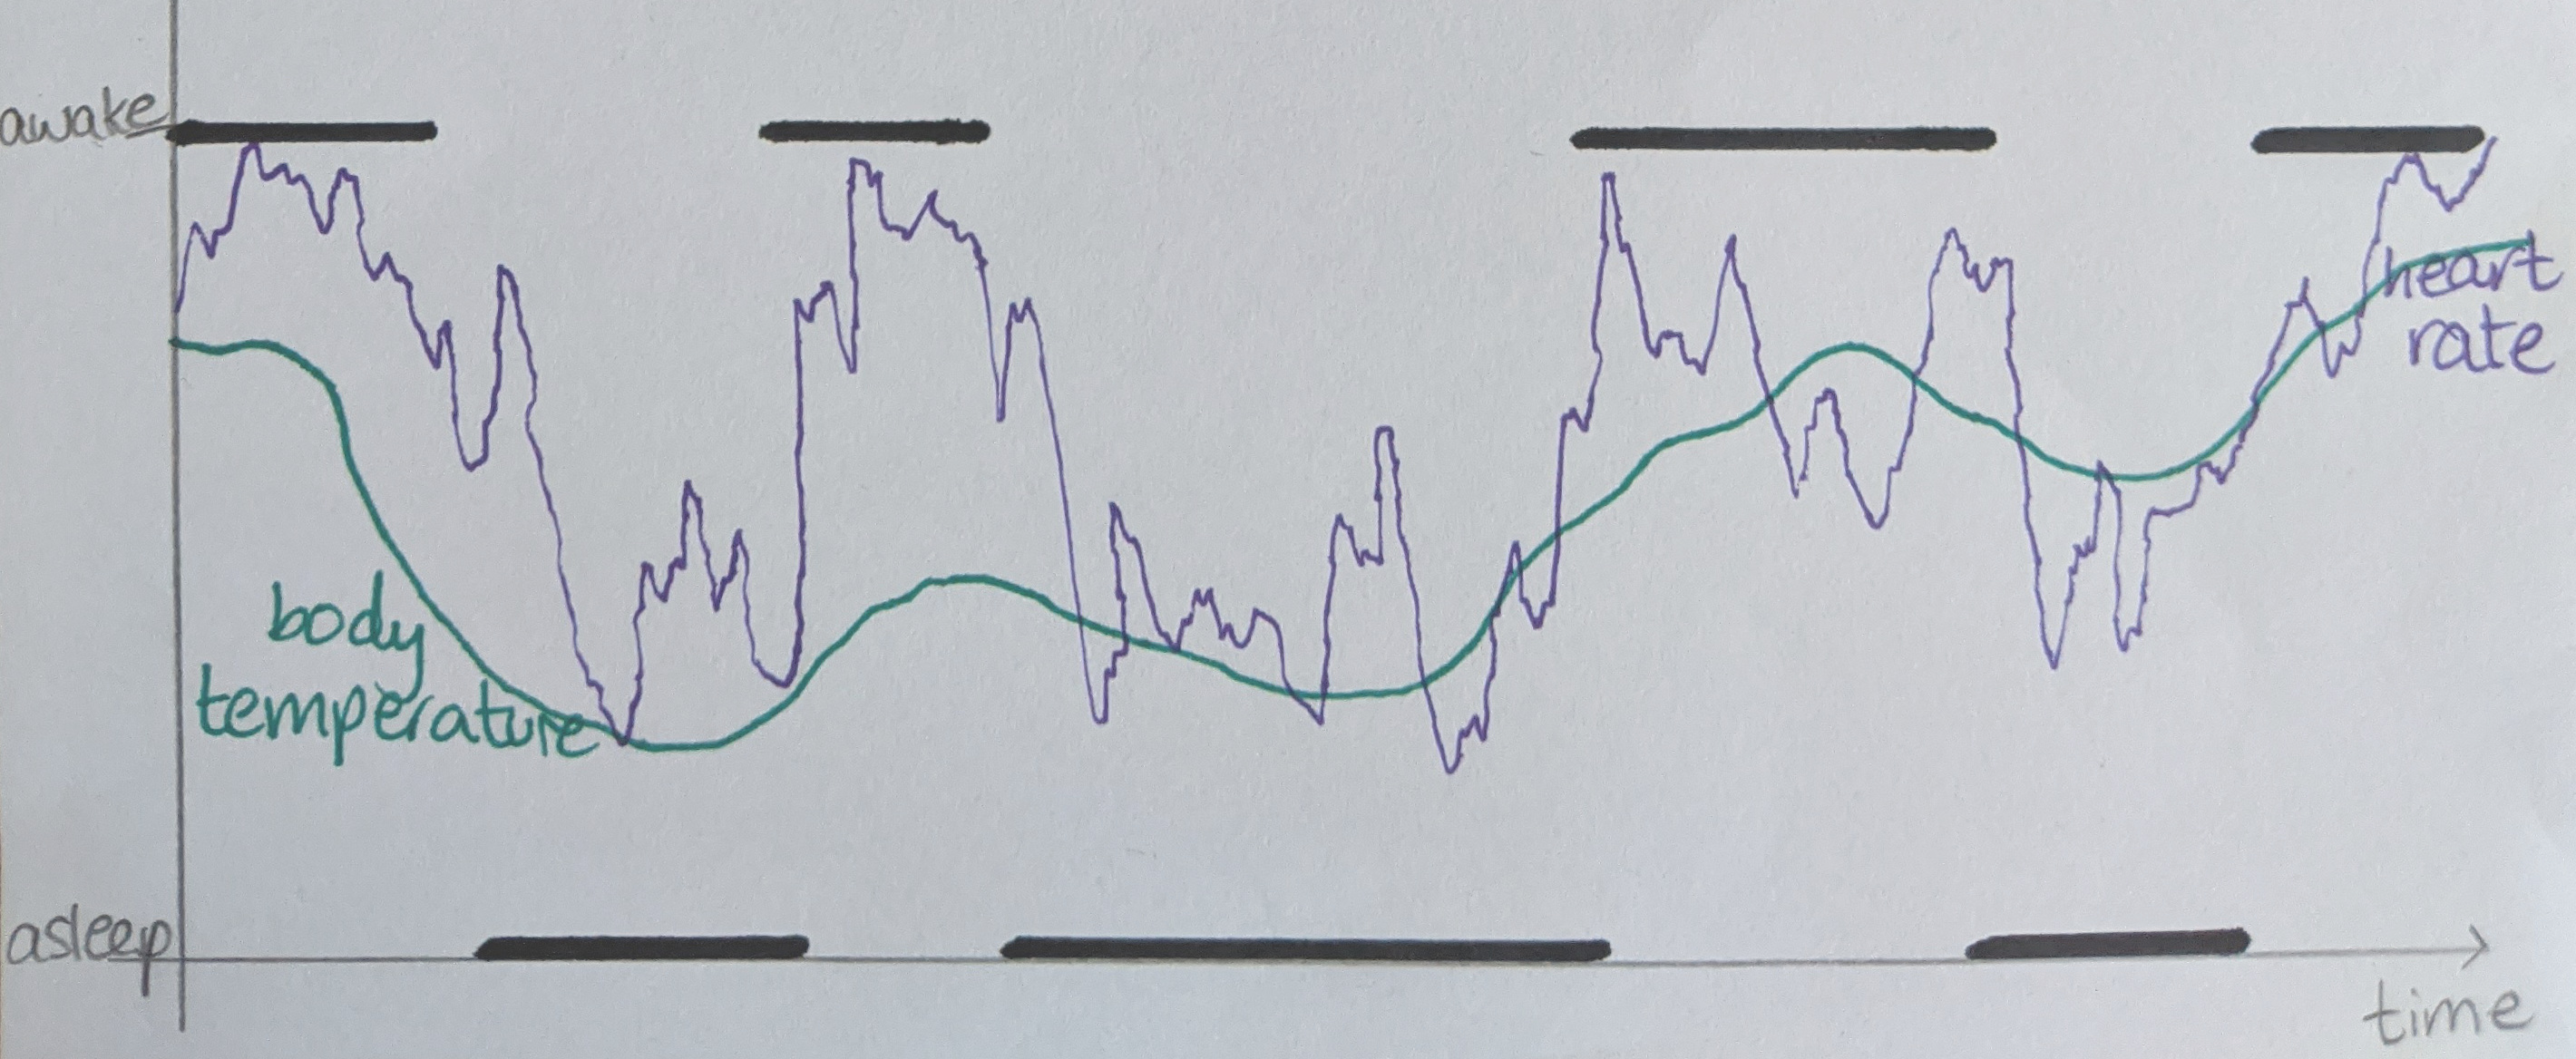
\includegraphics[width=0.8\textwidth]{ssm_ex_2.jpg}
%
%%%% NOTES
%% The example is in continuous time, but can easily imagine discrete observations (in fact only possible to get discrete obs!)
%% Model X as a Markov process with two states (so just need to choose switching rates/probabilities)
%% Also have some model for how temperature and heart rate vary with sleep
%% Actually this is a terrible example because it hardly makes sense to assume that Y_{t+1} depends on Y_t only via X...
%\end{frame}

\begin{frame}{Importance sampling}
\centering
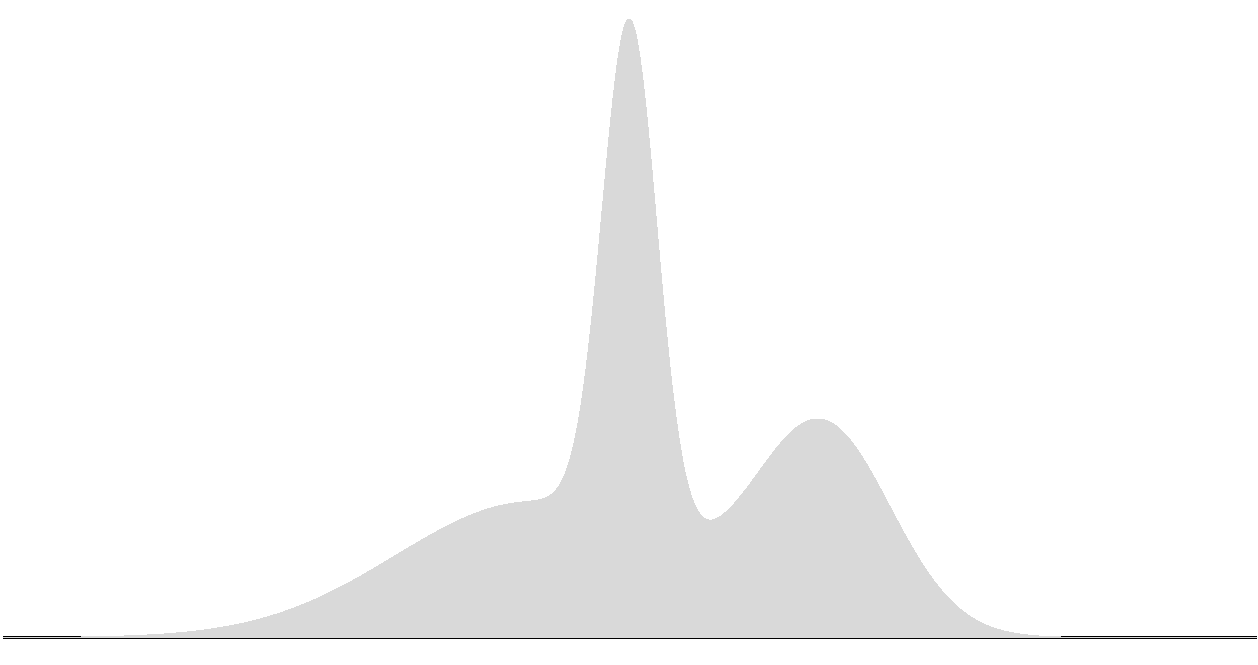
\includegraphics[width=0.9\textwidth]{importance1.pdf}

%%% NOTES
% Here's our "intractable" target
\end{frame}

\begin{frame}{Importance sampling}
\centering
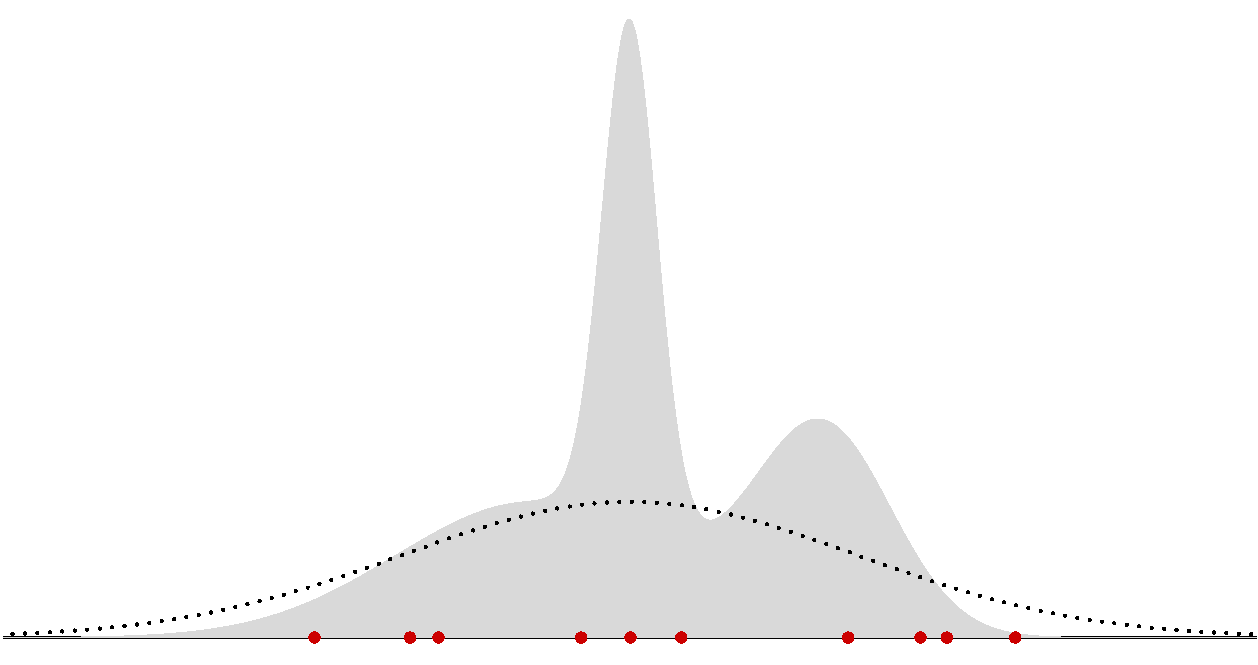
\includegraphics[width=0.9\textwidth]{importance2.pdf}

%%% NOTES
% Select a proposal density that we *can* sample from, and sample from it
\end{frame}

\begin{frame}{Importance sampling}
\centering
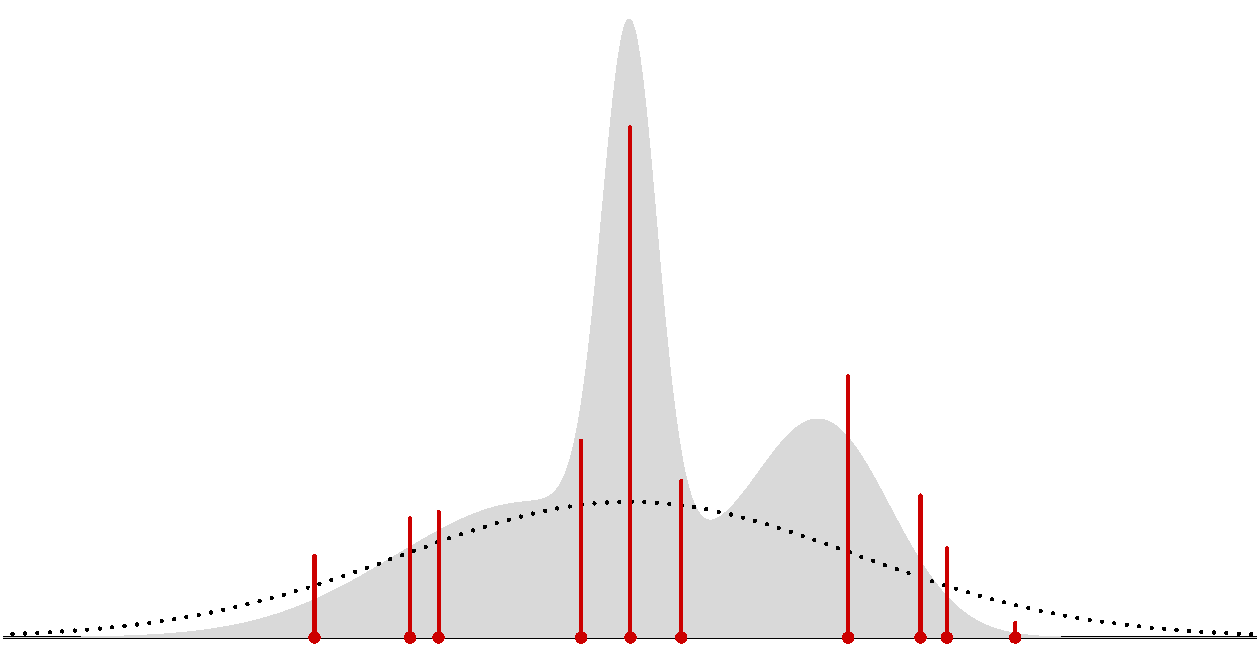
\includegraphics[width=0.9\textwidth]{importance3.pdf}

%%% NOTES
% Calculate weights for each sample proportional to ratio of target/proposal density 
% "The weighted samples are distributed according to the target" (in the sense that expectations are unbiased)
% We only needed to evaluate the target density pointwise up to a constant (standard assumption for Monte Carlo)
\end{frame}


\begin{frame}{Sequential importance sampling}
% Would be nice to remake this diagram as one that is more intuitively linked to the importance sampling one
\begin{itemize}
\item Idea: use weighted samples from one time step to construct a proposal for the next step
\item Multiplying weights over time causes \textit{weight degeneracy}% would be great to have an animation illustrating this...
\item Can avoid this problem by resampling (weights are reset at each step)

%%% NOTES
% Compounding time steps, get `particles' each with position and weight evolving over time
% SIS is a valid Monte Carlo algorithm
% Weight degeneracy = variance of weights explodes / all weight assigned to one particle
% Instead of taking weighted samples as proposal, make copies of samples according to weight, and reset weights to uniform
% SIR is also a valid algorithm!
\end{itemize}

\end{frame}


\begin{frame}{Resampling}
% Possibly include in this slide the 3 rules for valid resampling, if relevant later
\begin{columns}
\begin{column}{0.45\textwidth}
\begin{itemize}
\item Want to transform continuous weights to discrete offspring counts
\item For example, sample counts from Multinomial distribution 
\end{itemize}
\end{column}
\begin{column}{0.45\textwidth}
\centering
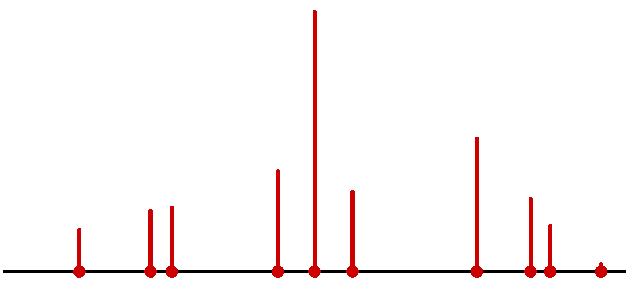
\includegraphics[width=\textwidth]{resample1.pdf} \\
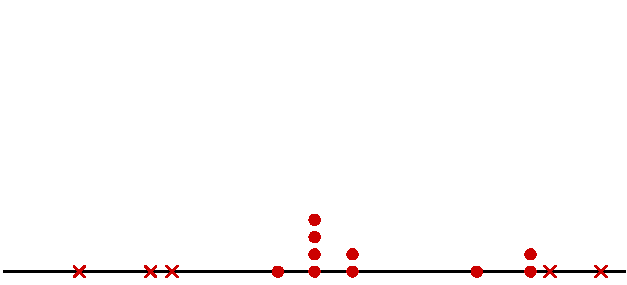
\includegraphics[width=\textwidth]{resample2.pdf}
\end{column}
\end{columns}

%%% NOTES
% Some particles will now start in the same positions, but they will be randomly moved (say with f_t) to construct the next proposal
\end{frame}


\begin{frame}{Sequential Monte Carlo algorithm}
Iterate these steps:
\begin{enumerate}
\item Mutate: move particle positions (according to $f_t$)
\item Weight: Calculate importance weights for each particle
\item Resample: Duplicate/kill particles according to weights, reset weights to $1/N$
\end{enumerate}
\end{frame}


\begin{frame}{Ancestral degeneracy}
\centering
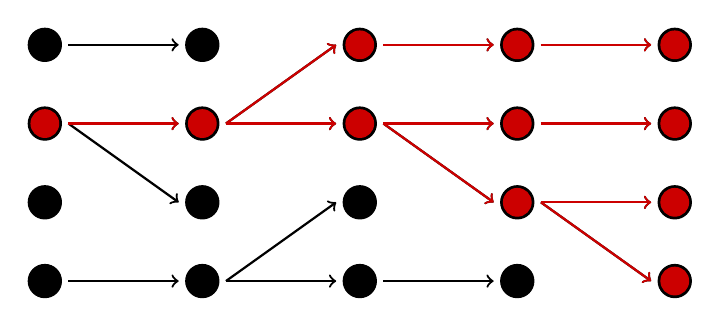
\begin{tikzpicture}
\filldraw (0,0) circle (6pt);
\filldraw (0,-1) circle (6pt);
\filldraw (0,-2) circle (6pt);
\filldraw (0,-3) circle (6pt);

\draw[->, thick] (0.3,0)--(1.7,0);
\draw[->, thick] (0.3,-1)--(1.7,-1);
\draw[->, thick] (0.3,-3)--(1.7,-3);
\draw[->, thick] (0.3,-1)--(1.7,-2);

\filldraw (2,0) circle (6pt);
\filldraw (2,-1) circle (6pt);
\filldraw (2,-2) circle (6pt);
\filldraw (2,-3) circle (6pt);

\pause

\filldraw (4,0) circle (6pt);
\filldraw (4,-1) circle (6pt);
\filldraw (4,-2) circle (6pt);
\filldraw (4,-3) circle (6pt);

\draw[->, thick] (2.3,-1)--(3.7,0);
\draw[->, thick] (2.3,-1)--(3.7,-1);
\draw[->, thick] (2.3,-3)--(3.7,-2);
\draw[->, thick] (2.3,-3)--(3.7,-3);

\pause

\filldraw (6,0) circle (6pt);
\filldraw (6,-1) circle (6pt);
\filldraw (6,-2) circle (6pt);
\filldraw (6,-3) circle (6pt);

\filldraw (8,0) circle (6pt);
\filldraw (8,-1) circle (6pt);
\filldraw (8,-2) circle (6pt);
\filldraw (8,-3) circle (6pt);

\draw[->, thick] (4.3,0)--(5.7,0);
\draw[->, thick] (4.3,-1)--(5.7,-1);
\draw[->, thick] (4.3,-1)--(5.7,-2);
\draw[->, thick] (4.3,-3)--(5.7,-3);

\draw[->, thick] (6.3,0)--(7.7,0);
\draw[->, thick] (6.3,-1)--(7.7,-1);
\draw[->, thick] (6.3,-2)--(7.7,-2);
\draw[->, thick] (6.3,-2)--(7.7,-3);

\pause
% highlight first lineage
\filldraw[darkred] (8,0) circle (5pt);
\filldraw[darkred] (6,0) circle (5pt);
\filldraw[darkred] (4,0) circle (5pt);
\filldraw[darkred] (2,-1) circle (5pt);
\filldraw[darkred] (0,-1) circle (5pt);

\draw[->, thick, darkred] (0.3,-1)--(1.7,-1);
\draw[->, thick, darkred] (2.3,-1)--(3.7,0);
\draw[->, thick, darkred] (4.3,0)--(5.7,0);
\draw[->, thick, darkred] (6.3,0)--(7.7,0);

\pause
% highlight other lineages
\filldraw[darkred] (4,-1) circle (5pt);
\filldraw[darkred] (6,-1) circle (5pt);
\filldraw[darkred] (8,-1) circle (5pt);
\filldraw[darkred] (6,-2) circle (5pt);
\filldraw[darkred] (8,-2) circle (5pt);
\filldraw[darkred] (8,-3) circle (5pt);

\draw[->, thick, darkred] (2.3,-1)--(3.7,-1);
\draw[->, thick, darkred] (4.3,-1)--(5.7,-1);
\draw[->, thick, darkred] (4.3,-1)--(5.7,-2);
\draw[->, thick, darkred] (6.3,-1)--(7.7,-1);
\draw[->, thick, darkred] (6.3,-2)--(7.7,-2);
\draw[->, thick, darkred] (6.3,-2)--(7.7,-3);
\end{tikzpicture}
\end{frame}


\begin{frame}{Ancestral degeneracy}
\centering
\vspace{1cm}
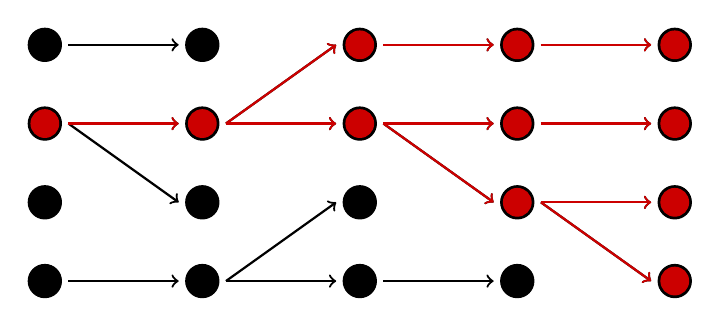
\begin{tikzpicture}
\filldraw (0,0) circle (6pt);
\filldraw (0,-1) circle (6pt);
\filldraw (0,-2) circle (6pt);
\filldraw (0,-3) circle (6pt);

\draw[->, thick] (0.3,0)--(1.7,0);
\draw[->, thick] (0.3,-1)--(1.7,-1);
\draw[->, thick] (0.3,-3)--(1.7,-3);
\draw[->, thick] (0.3,-1)--(1.7,-2);

\filldraw (2,0) circle (6pt);
\filldraw (2,-1) circle (6pt);
\filldraw (2,-2) circle (6pt);
\filldraw (2,-3) circle (6pt);

\filldraw (4,0) circle (6pt);
\filldraw (4,-1) circle (6pt);
\filldraw (4,-2) circle (6pt);
\filldraw (4,-3) circle (6pt);

\draw[->, thick] (2.3,-1)--(3.7,0);
\draw[->, thick] (2.3,-1)--(3.7,-1);
\draw[->, thick] (2.3,-3)--(3.7,-2);
\draw[->, thick] (2.3,-3)--(3.7,-3);

\filldraw (6,0) circle (6pt);
\filldraw (6,-1) circle (6pt);
\filldraw (6,-2) circle (6pt);
\filldraw (6,-3) circle (6pt);

\filldraw (8,0) circle (6pt);
\filldraw (8,-1) circle (6pt);
\filldraw (8,-2) circle (6pt);
\filldraw (8,-3) circle (6pt);

\draw[->, thick] (4.3,0)--(5.7,0);
\draw[->, thick] (4.3,-1)--(5.7,-1);
\draw[->, thick] (4.3,-1)--(5.7,-2);
\draw[->, thick] (4.3,-3)--(5.7,-3);

\draw[->, thick] (6.3,0)--(7.7,0);
\draw[->, thick] (6.3,-1)--(7.7,-1);
\draw[->, thick] (6.3,-2)--(7.7,-2);
\draw[->, thick] (6.3,-2)--(7.7,-3);

% highlight first lineage
\filldraw[darkred] (8,0) circle (5pt);
\filldraw[darkred] (6,0) circle (5pt);
\filldraw[darkred] (4,0) circle (5pt);
\filldraw[darkred] (2,-1) circle (5pt);
\filldraw[darkred] (0,-1) circle (5pt);

\draw[->, thick, darkred] (0.3,-1)--(1.7,-1);
\draw[->, thick, darkred] (2.3,-1)--(3.7,0);
\draw[->, thick, darkred] (4.3,0)--(5.7,0);
\draw[->, thick, darkred] (6.3,0)--(7.7,0);

% highlight other lineages
\filldraw[darkred] (4,-1) circle (5pt);
\filldraw[darkred] (6,-1) circle (5pt);
\filldraw[darkred] (8,-1) circle (5pt);
\filldraw[darkred] (6,-2) circle (5pt);
\filldraw[darkred] (8,-2) circle (5pt);
\filldraw[darkred] (8,-3) circle (5pt);

\draw[->, thick, darkred] (2.3,-1)--(3.7,-1);
\draw[->, thick, darkred] (4.3,-1)--(5.7,-1);
\draw[->, thick, darkred] (4.3,-1)--(5.7,-2);
\draw[->, thick, darkred] (6.3,-1)--(7.7,-1);
\draw[->, thick, darkred] (6.3,-2)--(7.7,-2);
\draw[->, thick, darkred] (6.3,-2)--(7.7,-3);
\end{tikzpicture}

\vspace{1cm}
For $t<<T$, $p(x_{1:t} | y_{1:T})$ is approximated by very few distinct points!
\end{frame}

\begin{frame}{Ancestral degeneracy}
\begin{itemize}
\item In smoothing applications, ancestral degenracy can seriously limit the performance of SMC
\item Can be mitigated by resampling less often (e.g.\ only when variance of weights gets too big --- ``adaptive resampling'')
\item Can also use low-variance resampling schemes
\item If we knew how bad ancestral degeneracy would be, we could tune parameters to limit it (e.g.\ number of particles, threshold for adaptive resampling)
\item Our aim: quantify ancestral degeneracy by analysing the induced genealogy
\end{itemize}
\end{frame}


\begin{frame}{Coalescence Probability}{Definition}
The probability that a randomly chosen pair of particles at generation $t$ share a common ancestor at generation $(t-1)$, conditional on offspring counts
\begin{equation*}
c_N = \frac{1}{N(N-1)} \sum_{i=1}^N \vt{i}(\vt{i}-1)
\end{equation*}

%%% NOTES
% N(N-1) is the number of pairs from which we choose uniformly
% the sum is over all possible parents that could be a common ancestor for the pair
% v_i(v_i-1) =0 if that parent had only one child, and is the number of ways this pair could be chosen from the i^th parent's offspring.
\end{frame}


%
% Add more frames here
%


\begin{frame}
\centering
THE END
\end{frame}
\end{document}